\section{制御雑音}
\begin{figure}[H]
\begin{center}
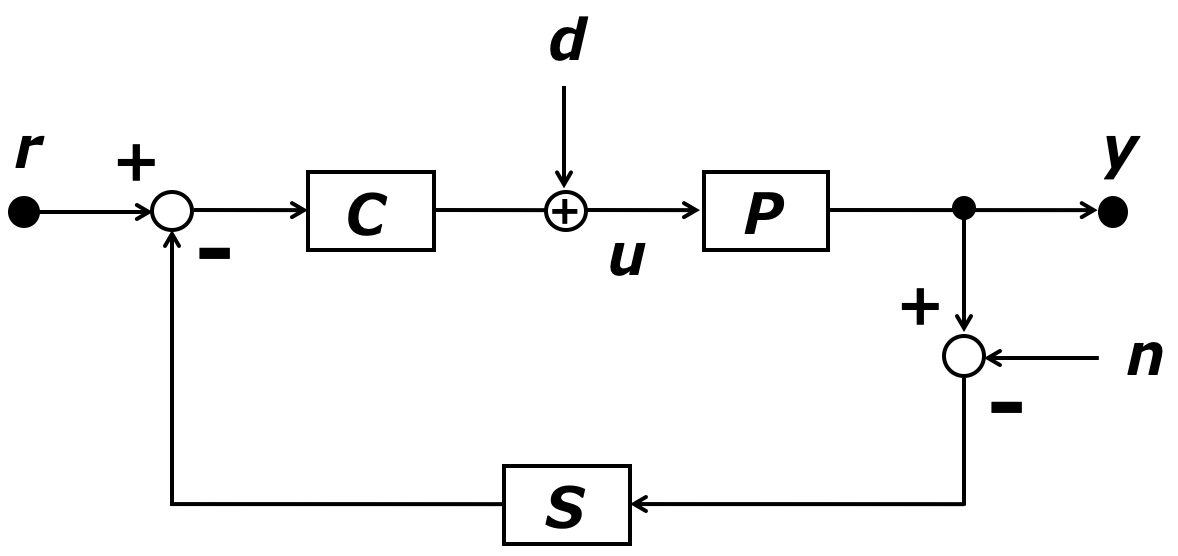
\includegraphics[width=120mm]{fig7_1.png}
\caption[制御雑音]{制御系には外乱と雑音が存在する. 図中の$d$は外乱, $n$は雑音, $r$は目標値, $y$は制御量を表す. }
\label{fig7.1}
\end{center}
\end{figure}
図\ref{fig7.1}において, 一巡伝達関数を$T_{\rm loop}=T_{\rm open}S=CPS$と書くと, 外乱$d$から制御量$y$, 雑音$n$から制御量$y$までの伝達関数はそれぞれ
\begin{equation}
T_{dy}\equiv\frac{y}{d}=\frac{P}{1+T_{\rm loop}}, 
\label{eq7.1}
\end{equation}
\begin{equation}
T_{ny}\equiv\frac{y}{n}=\frac{T_{\rm loop}}{1+T_{\rm loop}}, 
\label{eq7.2}
\end{equation}
となる. また, 目標値$r$から制御量$y$の伝達関数を制御系の特性とすると, その値は
\begin{equation}
T_{ry}\equiv\frac{y}{r}=\frac{CP}{1+CPS}=\frac{CP}{1+T_{\rm loop}}, 
\end{equation}
である. ここで, 制御対象が$P\rightarrow P+\Delta P$となったとき, 制御系の特性の変動は
\begin{equation}
\Delta T_{ry}=\frac{\Delta P}{1+C(P+\Delta P)S}\times\frac{T_{ry}}{P}, 
\label{eq7.4}
\end{equation}
となる. このとき微分感度は
\begin{equation}
S_0=\lim_{\Delta P\rightarrow 0}\frac{\Delta T_{ry} / T_{ry}}{\Delta P / P}, 
\label{eq7.5}
\end{equation}
と定義される. ただし, $\frac{\Delta T_{ry} / T_{ry}}{\Delta P / P}$は相対感度と呼ばれ, この値が1より小さい時は外乱に対して制御特性が変動しにくいことを意味している. \\
\quad 式(\ref{eq7.4}), (\ref{eq7.5})より, 
\begin{equation}
S_0=\lim_{\Delta P\rightarrow 0}\frac{\left(\frac{\Delta P}{1+C(P+\Delta P)S}\times\frac{T_{ry}}{P}\right) / T_{ry}}{\Delta P / P}=\frac{1}{1+CPS}=\frac{1}{1+T_{\rm loop}}, 
\label{eq7.6}
\end{equation}
と書くことができるので, 式(\ref{eq7.1})より
\begin{equation}
T_{dy}=S_0P, 
\label{eq7.7}
\end{equation}
である. また, 式(\ref{eq7.2})から
\begin{equation}
S_0+T_{ny}=1, 
\label{eq7.8}
\end{equation}
と書ける. このとき, 外乱の影響を小さくする, すなわち$T_{dy}$を小さくしようとすると式(\ref{eq7.7})より, $S_0$も小さくなる. すると式(\ref{eq7.8})より, $T_{ny}$が大きくなる. \\
\quad つまり, ダンピングフィルタをかけて振動を抑えようとする(=外乱を抑えようとする)と雑音の影響が大きくなってしまう. また, 逆に雑音を減らそうとすると外乱の影響が大きくなる. 例えば$S$にローパス特性を持たせる(=高周波帯において$T_{\rm loop}$を小さくする)などしても, 式(\ref{eq7.6})より$S_0$が大きくなるため, 式(\ref{eq7.7})より$T_{dy}$も大きくなるのである. \\
\quad このように, ダンピング制御と雑音はトレードオフの関係にある. よって, 低周波帯では振動減衰を, 高周波帯では雑音低減を重視するというような制御がよく用いられる. \\
\quad しかし, 図\ref{fig3.7}に示したLock-acquisition PhaseではFP共振器を素早くロックすることが目標であるため, 広い帯域で強い制御をかける必要がある. 一方, Observation Phaseにおいては安定な干渉計ロックを保持できるレベルの制御で十分であり、それよりも雑音の低減を目指すべきである. 前回の観測 (O3GK) では懸架系の制御がLock-acquisition Phase のままであったが, 本研究では, Observation Phaseにおける低雑音な制御を行うことを目標とした. 以下の節でそれを述べる. 
\section{制御フィルタの変更}
まず, Type-A suspensionのうち, ETMY, ITMX, ITMYの3つに対してObservation Phaseにおける制御フィルタ(以下Observation フィルタ)を作成した. ここではITMXについて実際のフィルタを示しながらその設計について記載する.
%まず, Observation Phaseにおける制御フィルタ(以下Observation フィルタ)を作成した. ただし, ETMXはテストマスに干渉計の信号がフィードバックされており, 干渉計の長さを決めている.そのため, FPMIの時点で制御を変えてしまうと, PRFPMIを構成した際に問題が生じる. よって本論文ではType-A suspensionのうち, ETMY, ITMX, ITMYの3つを低雑音制御の対象とする. 
\subsection{ITMX Length}
まずL方向について, フォトセンサの出力信号からダンプしすぎている周波数がないか確かめた(図\ref{fig7.2}). そして, そのスペクトルからどのくらいオーバーダンプしているかを見積もり, その分だけダンピングフィルタのゲインを下げた. さらに共振の位置にノッチフィルタを入れてピークを潰し, 10 Hz以上では4次の楕円ローパスフィルタによって, 従来以上に急峻にゲインを落とした(楕円フィルタは同じ次数を持った他のフィルタに比べて, ゲインの変化が最も早いという特性を持つフィルタである). その後1晩放置し, 信号が発振しないことを確かめた. 最終的なフィルタは図\ref{fig7.3}の通りである.
\begin{figure}[H]
\begin{center}
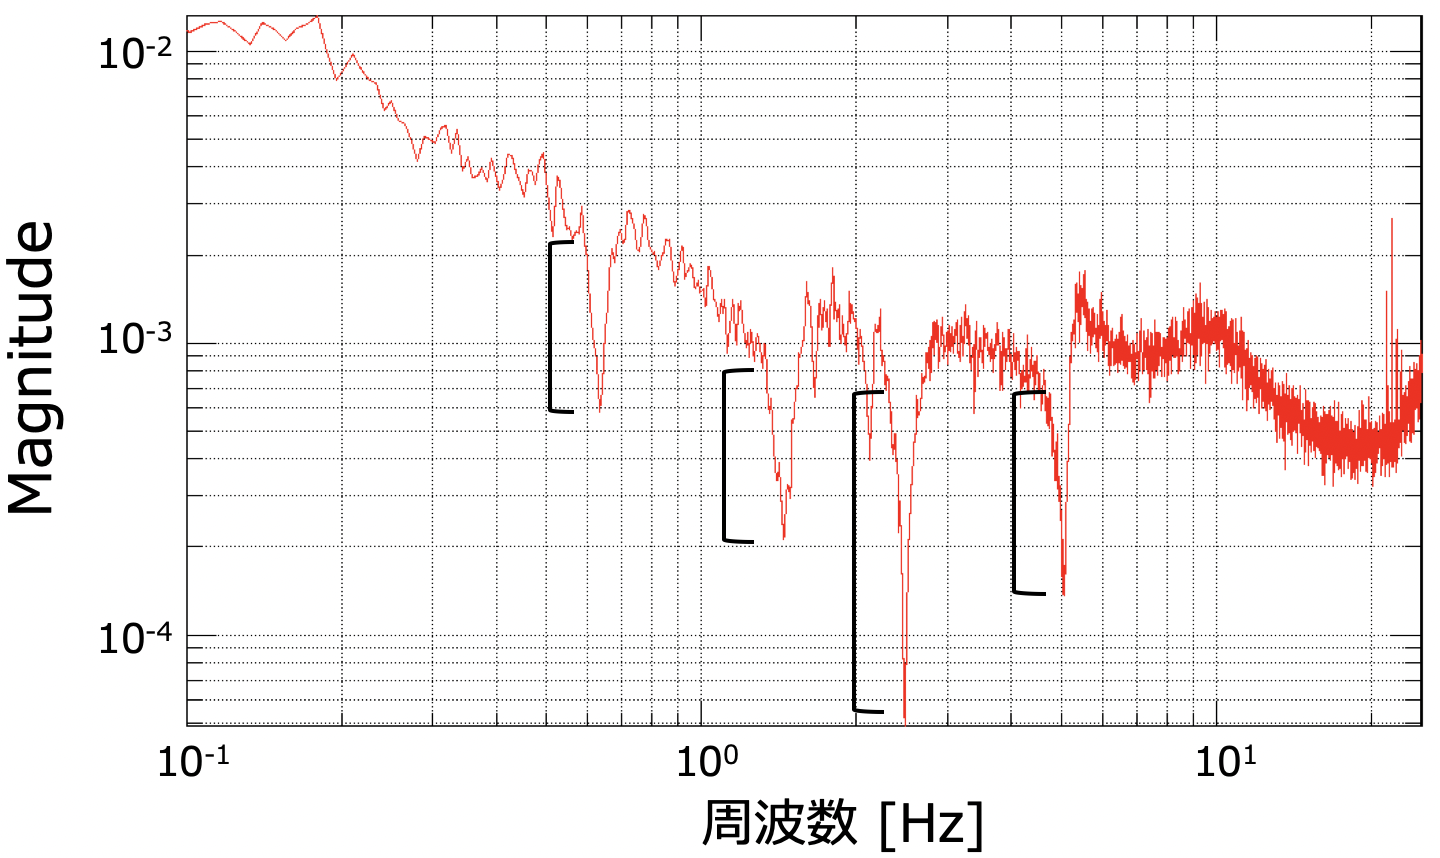
\includegraphics[width=140mm]{fig7_2.png}
\caption[フォトセンサのエラー信号 (ITMX MN L)]{フォトセンサのエラー信号 (ITMX MN L). 落ち込んでいる部分が共振ピークでの揺れをダンピングしている箇所であり, エラー信号のレベルに対してどの程度小さくなっているかという値からオーバーダンプの度合いを見積もっている.}
\label{fig7.2}
\end{center}
\end{figure}
\begin{figure}[H]
\begin{center}
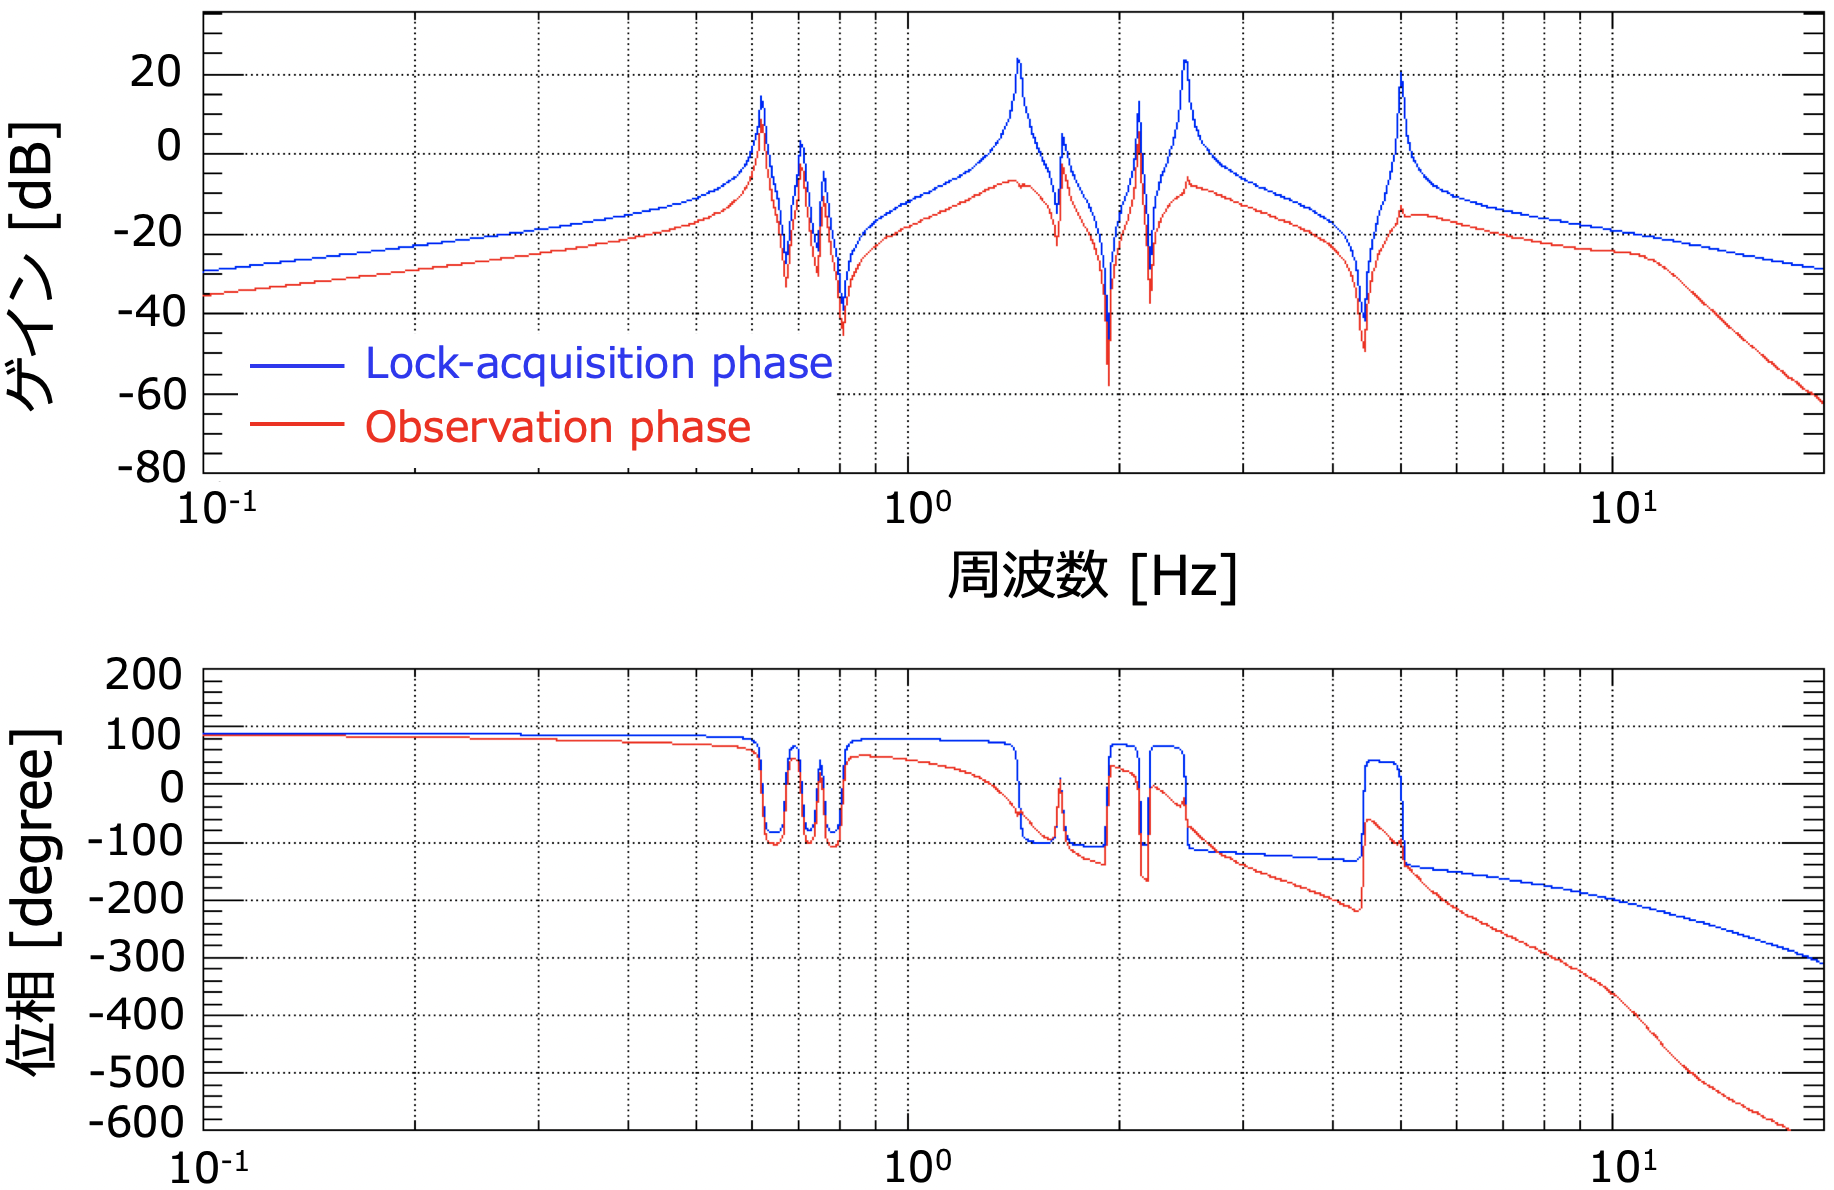
\includegraphics[width=160mm]{fig7_3.png}
\caption[Observation フィルタ (ITMX L)]{赤線がObservation フィルタ (ITMX L), 青線がLock-acquisition phaseで用いられるフィルタをかけた時のMNの応答を表す. Lock-acquisition phaseで用いるフィルタよりもゲインを下げ, 共振ピークをノッチで潰した上, 10 Hz以上では楕円フィルタによって急峻にゲインを下げている.}
\label{fig7.3}
\end{center}
\end{figure}
\subsection{ITMX Pitch}
P, Y方向のフォトセンサのダンピング制御はObservation phaseでは完全にオフにし, OpLevを用いて制御を行う. これはP, Y方向に関しては, OpLevを用いた方が制御雑音が小さいことが分かっているからである. \\
\quad Lの場合と同様にしてゲインの下げ方を調べた. その結果0.2 Hz前後をUGFとしてゲインを下げればよいことが分かった. そこで, UGFでの位相の回りに注意しながら0.4 Hzから4次楕円ローパスフィルタをかけた. さらに共振の位置にノッチフィルタを入れてピークを潰し, しばらく放置して安定であることを確かめた.\\
\quad 実際に設計したフィルタを図\ref{fig7.4}に示す. 赤線がObservation フィルタを表しており, UGFは0.191 Hz, そこでの位相余裕は$21^{\circ}$となっている.
\begin{figure}[H]
\begin{center}
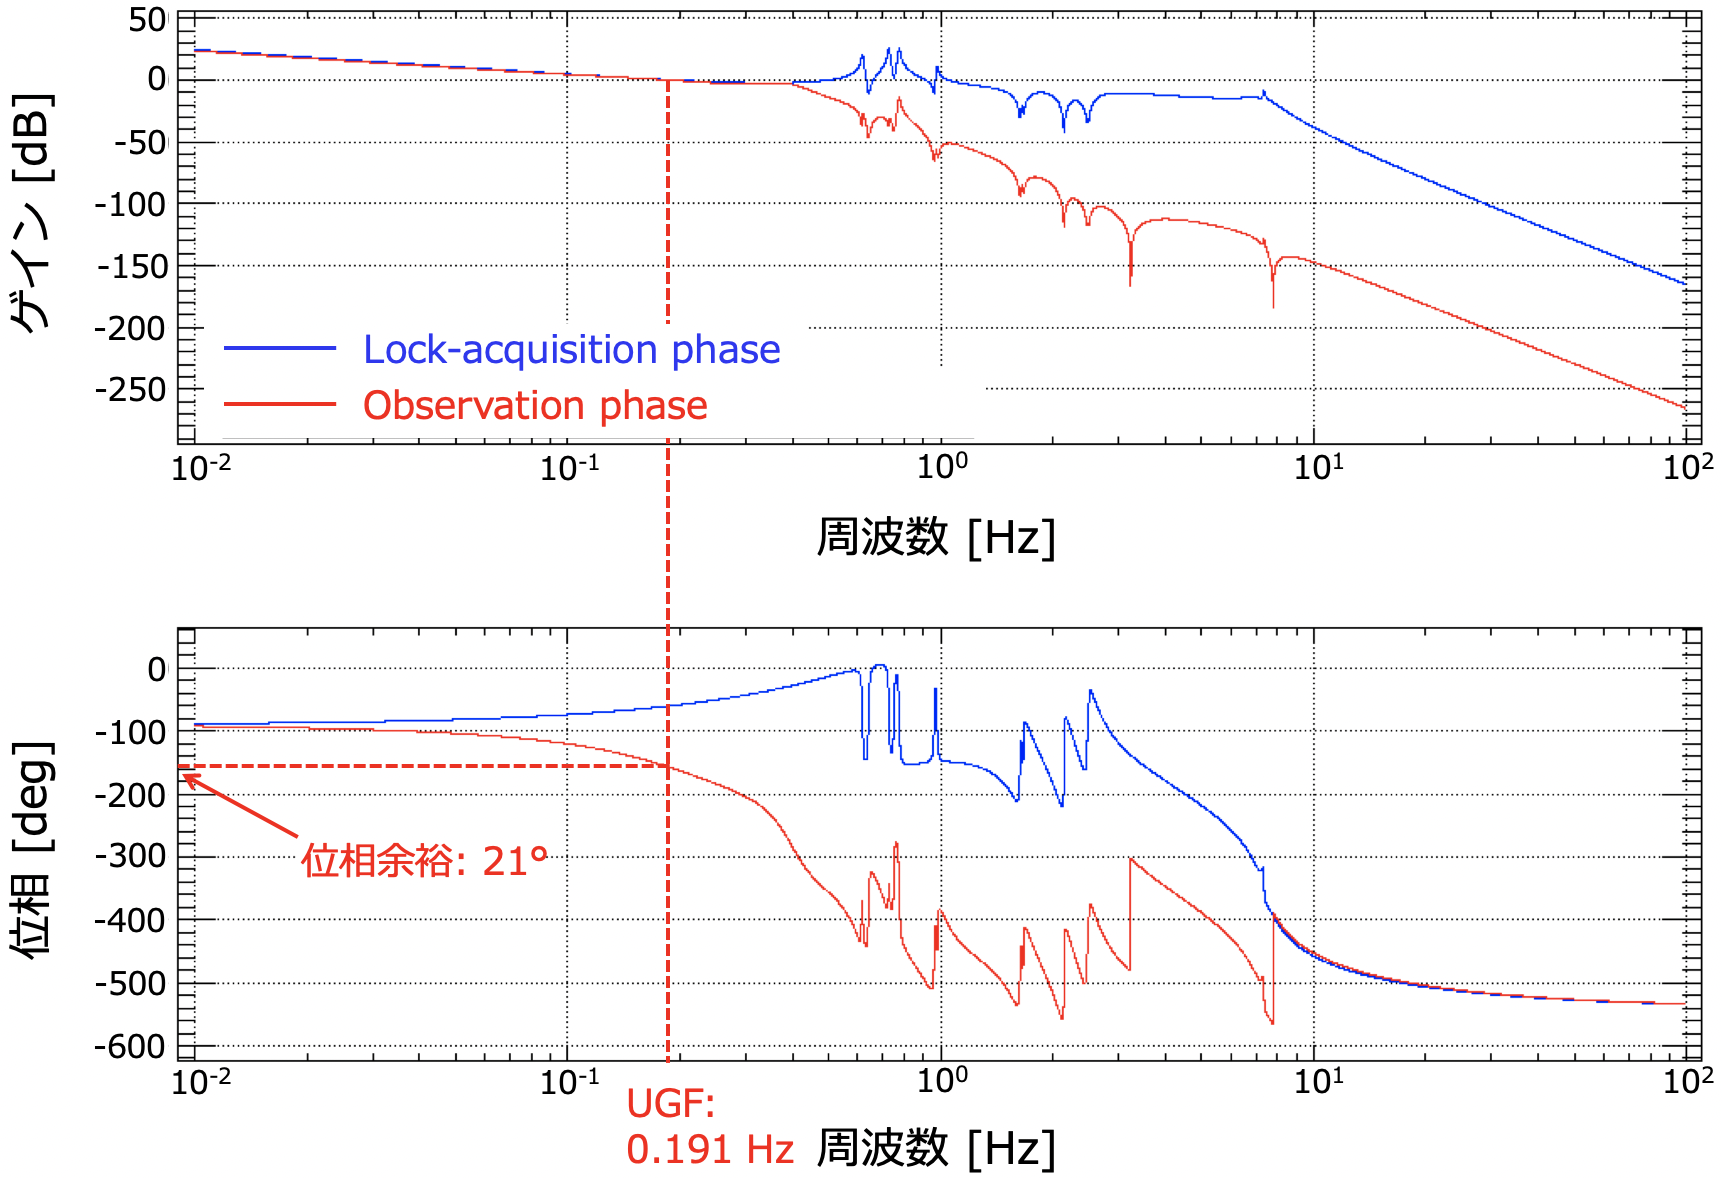
\includegraphics[width=170mm]{fig7_4.png}
\caption[Observation フィルタ (ITMX P)]{赤線がObservation フィルタ (ITMX P), 青線がLock-acquisition phaseで用いられるフィルタをかけたときのMNの応答を表す. なお, Observation フィルタについて, UGFは0.191 Hzであり, そこでの位相余裕は$21^{\circ}$である.}
\label{fig7.4}
\end{center}
\end{figure}
同様の制御をITMY, ETMYにも実装し, 制御雑音を測定した.
\section{制御雑音の測定}
\subsection{測定方法}
まずFPMI(第\ref{第2章}章参照)をロックする. このFPMIにおいて, 重力波信号は腕の差動信号であり, DARM信号と呼ばれている. また, DARM信号は図\ref{fig7.5}においてPDに向かって来るので, そこで取得される. その信号を用いてETMXにフィードバック信号を返し, 腕の差動変異を保つようにETMXを駆動している.
\begin{figure}[H]
\begin{center}
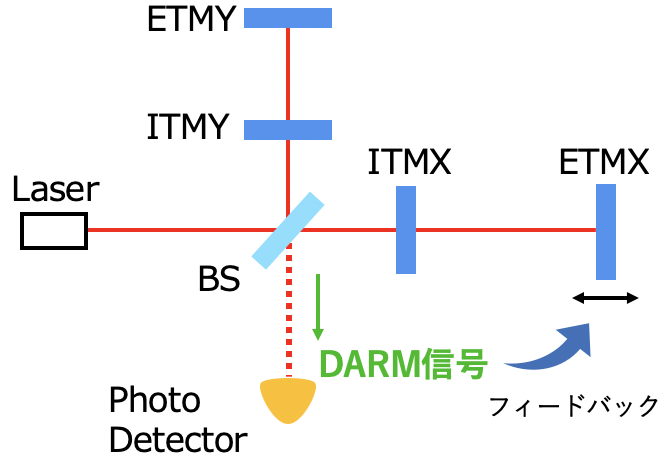
\includegraphics[width=120mm]{fig7_5.png}
\caption[FPMIの構成とDARM信号]{FPMIの構成とDARM信号}
\label{fig7.5}
\end{center}
\end{figure}
次に, 制御雑音を測定するために, 各懸架装置を各自由度に振動させ, その動きからDARM信号までの伝達関数を測定した. 測定した伝達関数の例を図\ref{fig7.6}に示す. 
\begin{figure}[H]
\begin{center}
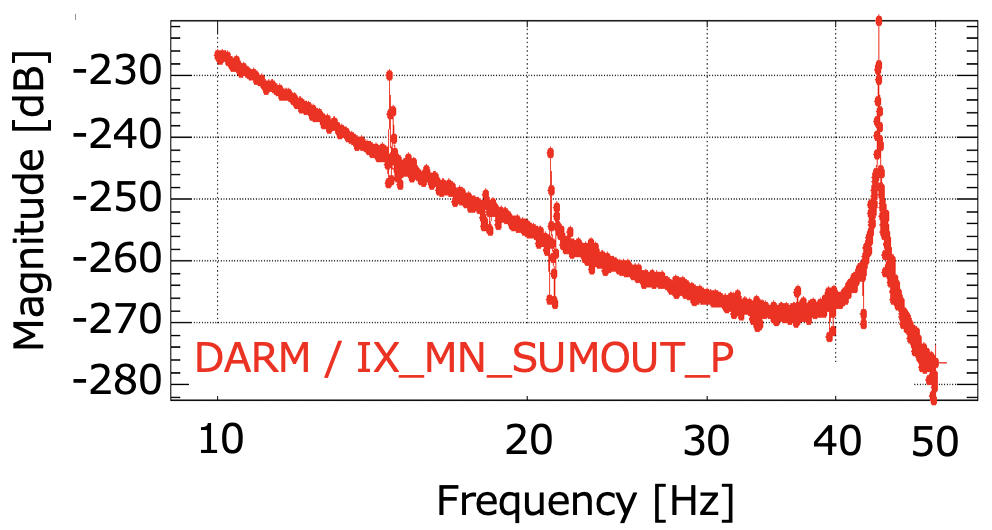
\includegraphics[width=120mm]{fig7_6.png}
\caption[ITMX MN Pの出力からDARM信号までの伝達関数]{ITMX MN Pの出力からDARM信号までの伝達関数}
\label{fig7.6}
\end{center}
\end{figure}
懸架装置をこのように振動させていない時でも, 制御に用いるセンサの雑音は常に存在している. そこで各自由度の出力の振幅スペクトル密度 (Amplitude Spectrum Density: ASD)  $S_{\rm SUMOUT}$を測定した伝達関数${\rm TF}_{\rm SUMOUT}$にかけることによって, 制御雑音が得られる. 
\begin{equation}
N_{\rm control}={\rm TF}_{\rm SUMOUT}\times S_{\rm SUMOUT}.
\end{equation}
さらに、各懸架装置の制御雑音は無相関であるから, ETMXを除くType-A suspensionの制御雑音の2乗和を取ることで, 全体の制御雑音が得られる. 
\begin{equation}
N_{\rm control, all}=\sqrt{N_{\rm control, ETMY}^2+N_{\rm control, ITMX}^2+N_{\rm control, ITMY}^2}.
\label{eq7.10}
\end{equation}
\subsection{測定結果}
作成したObservation フィルタを使用した場合と, しなかった場合について, 式(\ref{eq7.10})の計算をした結果を図\ref{fig7.7}に示した. 
\begin{figure}[H]
\begin{center}
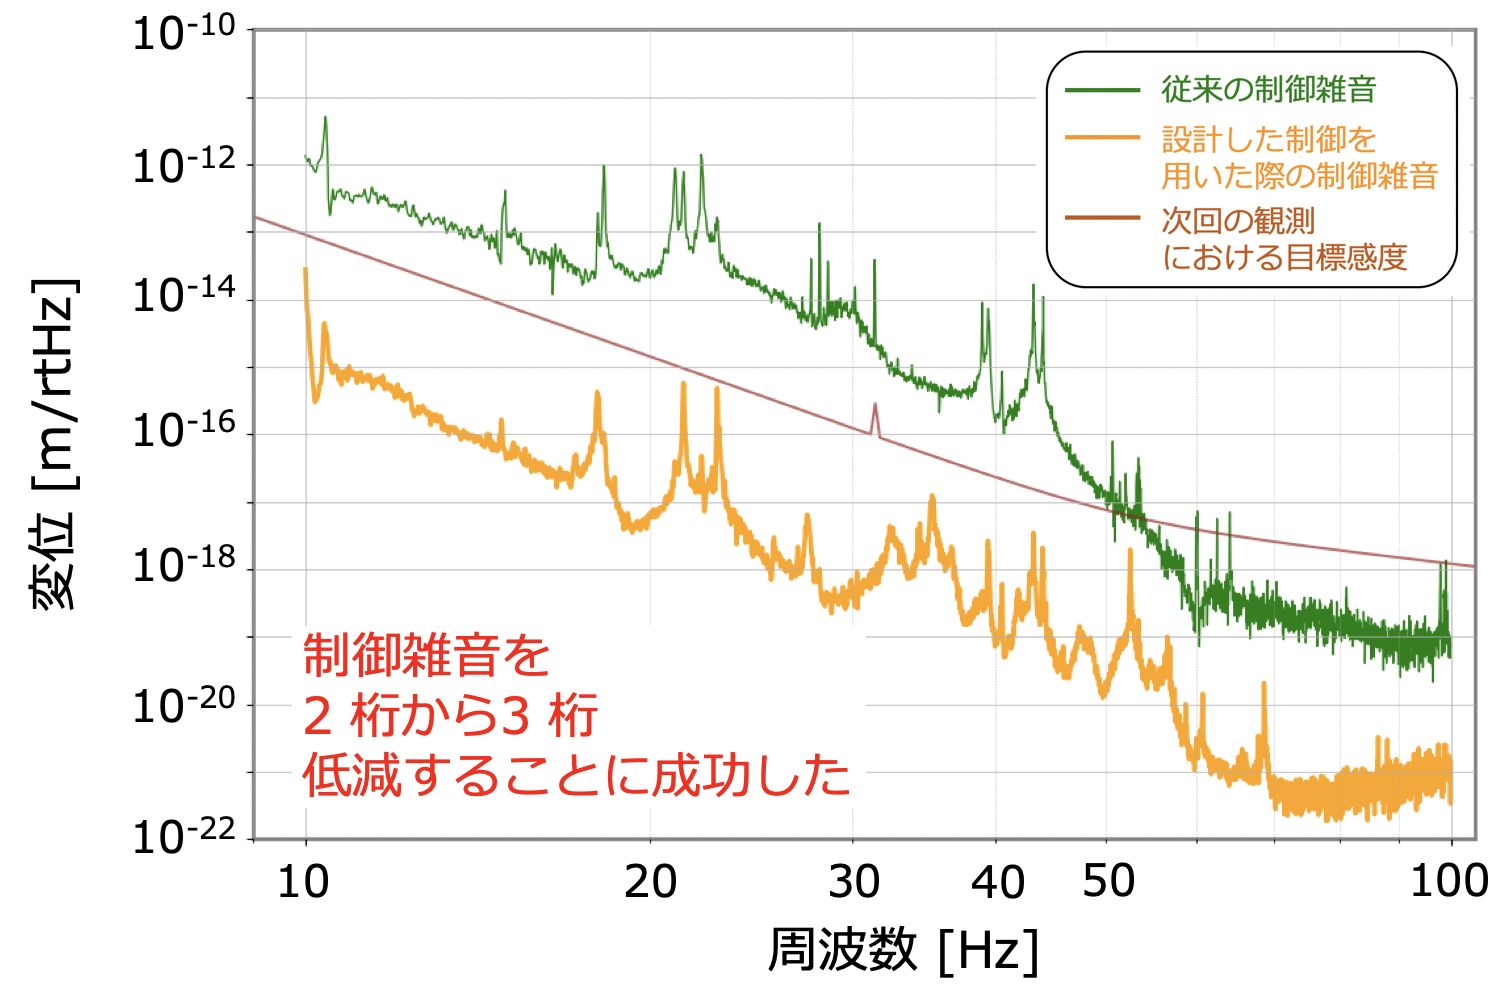
\includegraphics[width=160mm]{fig7_7.png}
\caption[Observation フィルタの効果]{Observation フィルタの効果. Observation フィルタを用いることにより, 低温懸架装置の制御雑音が$2\sim3$ 桁小さくなっており, これはO4a観測における目標感度 (3 Mpc) と比べても小さい. }
\label{fig7.7}
\end{center}
\end{figure}
図中の緑線がObservationフィルタなしの場合, オレンジの線がObservationフィルタありの場合を示している. これより, Observationフィルタを使用することで, ETMXを除く低温懸架装置の制御雑音が$2\sim3$ 桁小さくなっているのが分かる. また, Observationフィルタを使用した場合の制御雑音は, O4a観測(Observation 4の初めの段階)における目標感度 (3 Mpc) と比べても小さいと分かる.\\
\quad さらに, 図\ref{fig7.8}に現在のFPMIの感度(赤)とObservationフィルタありの場合の制御雑音(オレンジ), および各懸架装置の各自由度についての制御雑音を示した. これより, 幅広い帯域でETMYのYに対する制御雑音が支配的であることが分かる. また, この図に示された懸架装置の違いによる制御雑音の差を埋めることは, 今後の課題である.
\begin{figure}[H]
\begin{center}
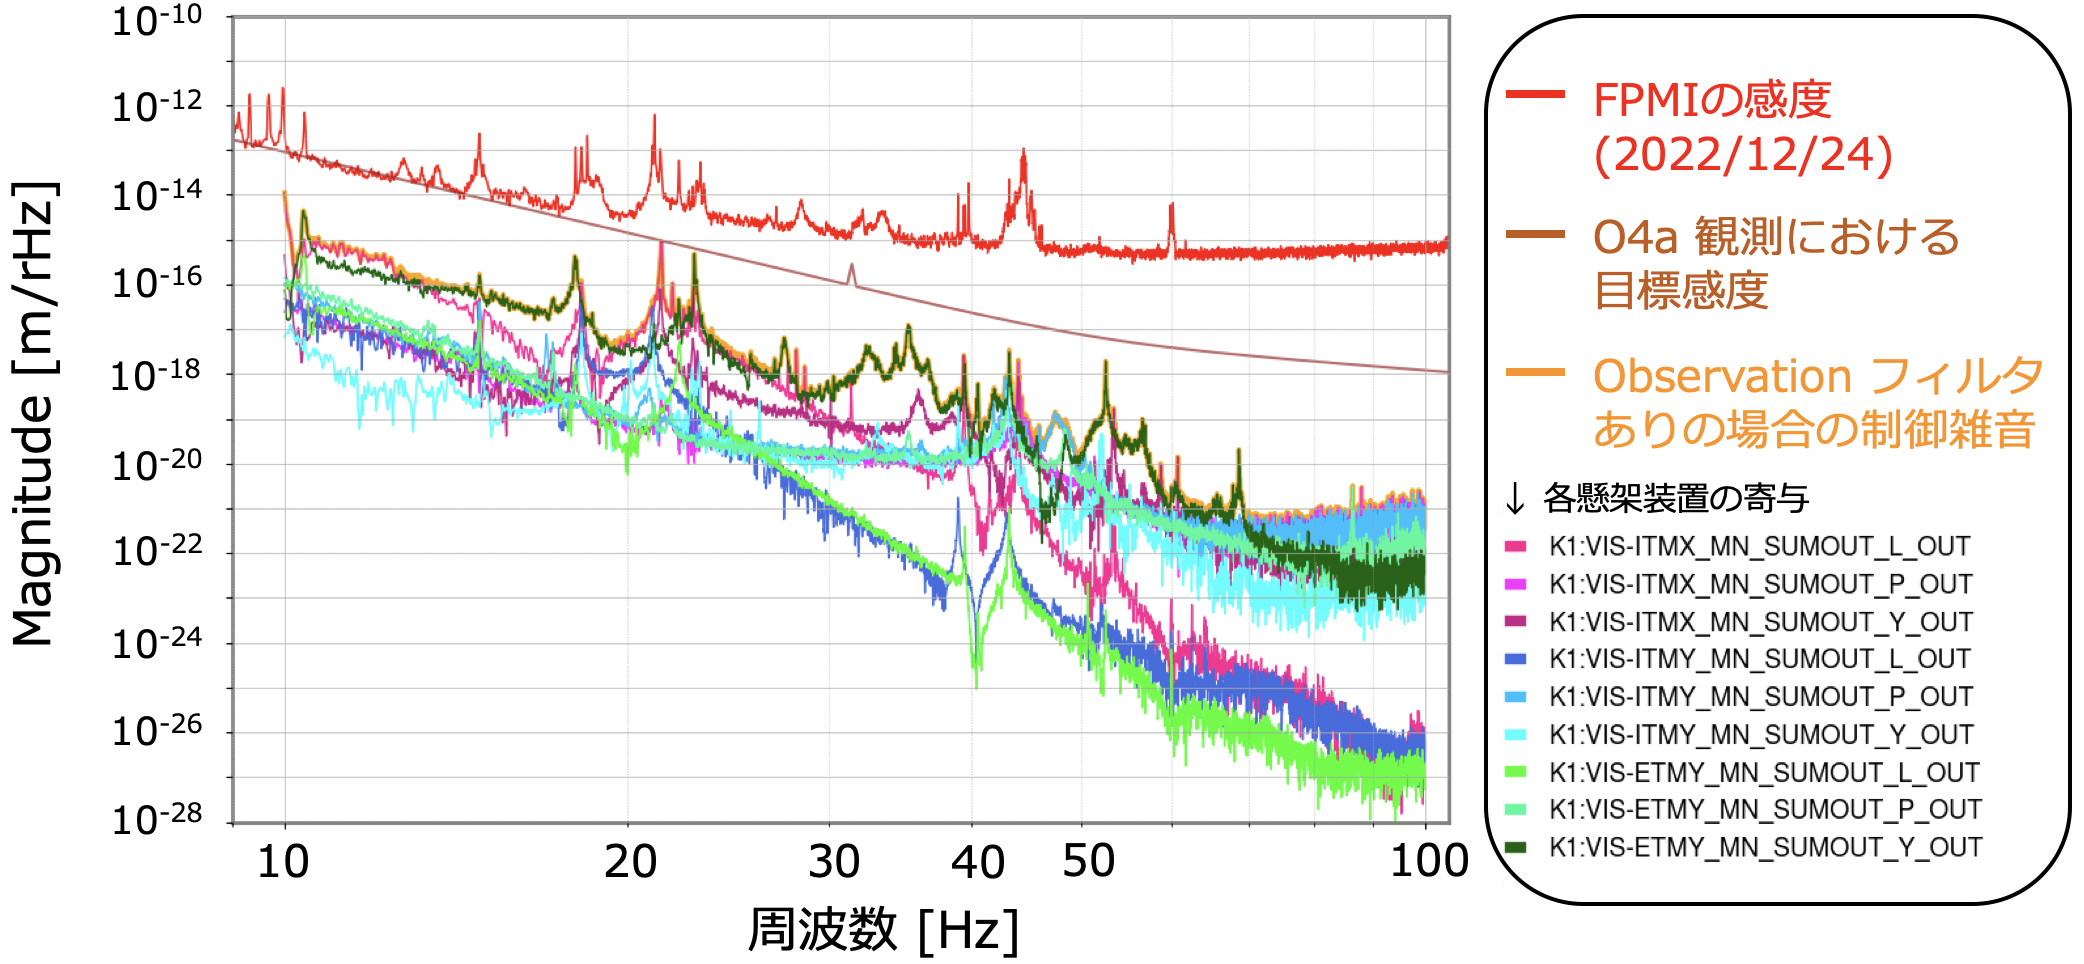
\includegraphics[width=160mm]{fig7_8.png}
\caption[懸架装置, 自由度ごとの制御雑音]{懸架装置, 自由度ごとの制御雑音. ETMYのYに対する制御が最も大きな雑音を生んでいる.}
\label{fig7.8}
\end{center}
\end{figure}
なお, 現在$10\sim50$ Hzにおいて, まだObservationフィルタを実装していないETMXの制御雑音が他の低温懸架装置と比べて著しく大きいでことは判明している(図\ref{fig7.9}). しかし, 本研究の成果より, ETMXに対しても同様の制御を実装すれば, O4観測にとって十分なレベルまで制御雑音を低減可能であると推察される.
\begin{figure}[H]
\begin{center}
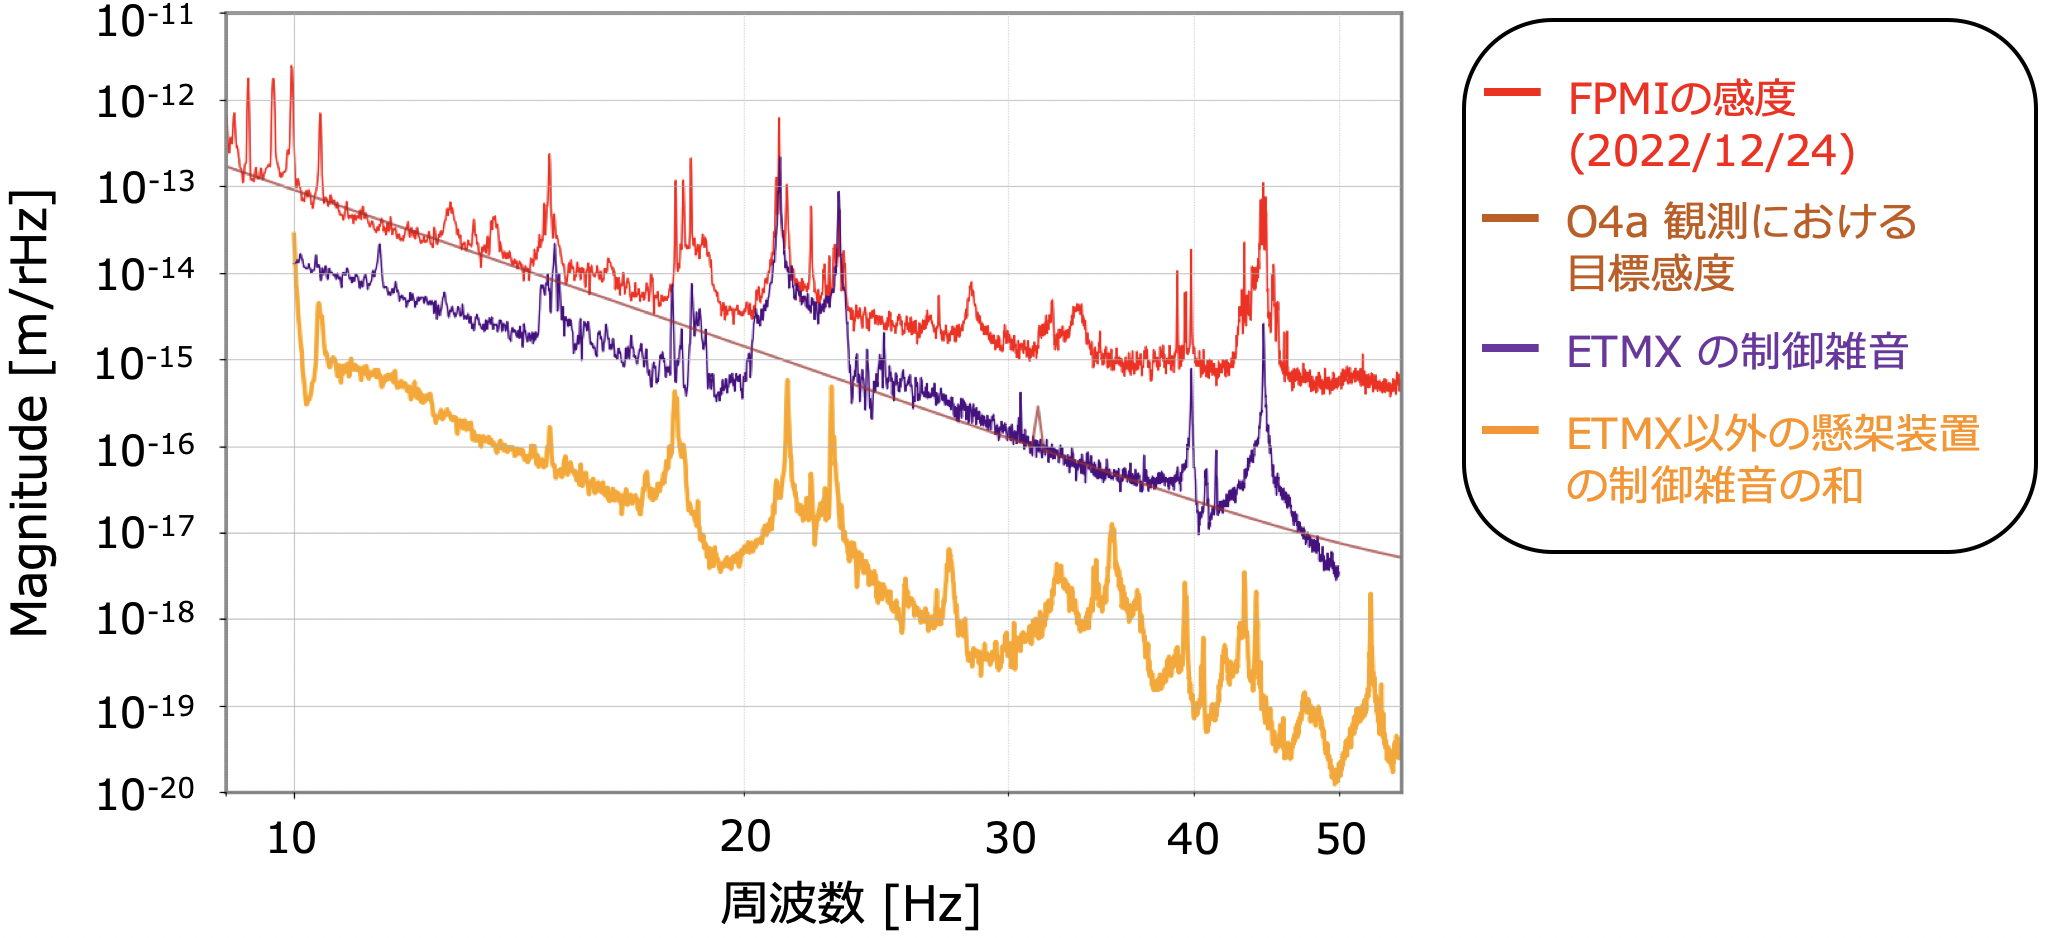
\includegraphics[width=160mm]{fig7_9.png}
\caption[ETMXの制御雑音]{ETMXの制御雑音. 現在はETMXの制御雑音が著しく大きい. しかし, 他の低温懸架装置と同様の制御を実装すれば, O4観測に十分なレベルまで制御雑音を低減できると考えられる.}
\label{fig7.9}
\end{center}
\end{figure}
また, 新たに設計した制御を用いてもFPMIが安定に動作するかどうかを確かめた. 図\ref{fig7.10}はその時の干渉計の状態を示している. 図中のFPMI Lockedは従来の制御フィルタを用いてFPMIをロックしている状態であり, Observationが低雑音制御に切り替えた状態である. 2023年1月4日の13時43分にFPMI LockedからObservationに切り替え, 2023年1月5日の13時46分までの約26 時間, FPMIが安定に動作することが確かめられた. なお, 2023年1月5日の13時46分にFPMIのロックを落としたのは, 干渉計作業のためであり, これは人為的なものである.
\begin{figure}[H]
\begin{center}
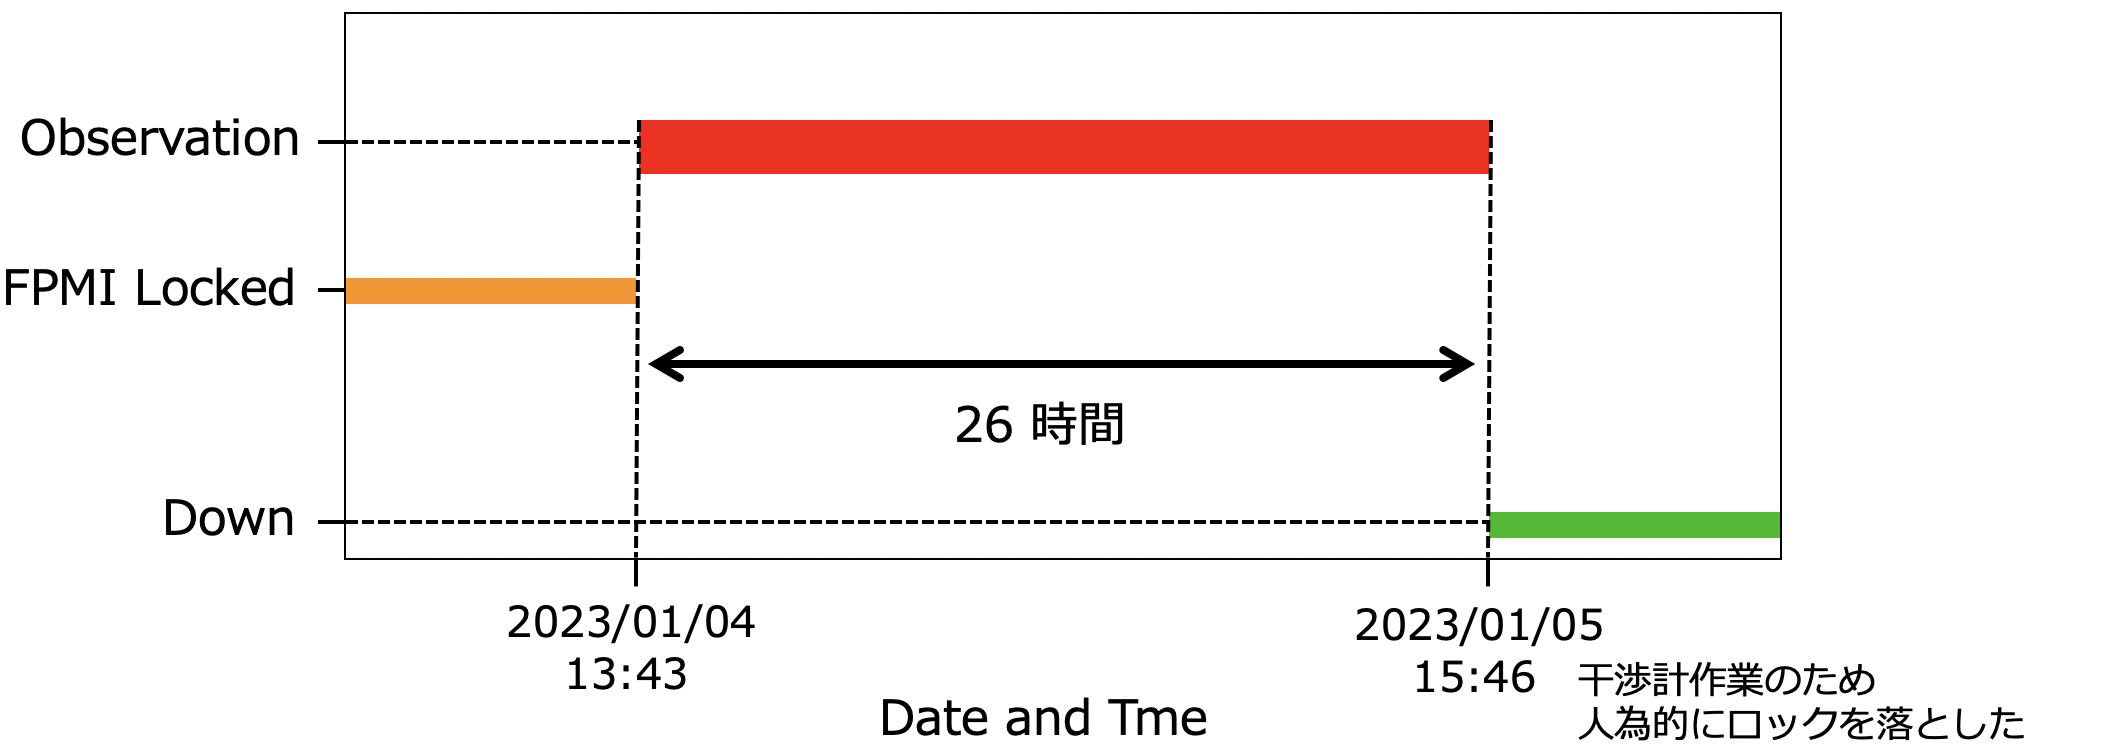
\includegraphics[width=160mm]{fig7_10.png}
\caption[FPMIの安定性]{Observatiobフィルタを用いた際のFPMIの安定性. FPMI Locked, Observationはそれぞれ従来の制御, 新しく設計した制御を用いてFPMIをロックしている状態である. 2023年1月4日の13時43分にFPMI LockedからObservationに切り替え, 人為的にロックを落とした2023年1月5日の13時46分までの約26 時間, FPMIが安定に動作することを確かめた.}
\label{fig7.10}
\end{center}
\end{figure}

\section{制御雑音低減のまとめ}
ETMY, ITMX, ITMYの低温懸架装置に対して制御雑音の低減を目指したObservation フィルタを作成し, $10\sim100$ Hzにおいて制御雑音を$2\sim3$ 桁低減することに成功した.  未実装のETMXに対しても同様の制御を行うことにより, O4観測における制御雑音低減の目標を完全に達成することが期待される. また, 新たに設計した制御を用いてもFPMIを長時間安定に動作できることを確認した. \\
\quad しかし, O5観測では128 Mpcが目標感度とされており, それを実現するためには低温懸架装置の制御雑音をさらに低減する必要がある. それを実現するためには様々なアプローチが考えられ, 例えば振動をモードごとに分解してそれらを独立に減衰させる手法などが考えられる. これにより, ダンピング性能と制御雑音の最適化が容易となり, 効率良く制御を行えるようになると期待できる\cite{modal}. あるいは, 現在ダンピング制御に用いられているフォトセンサよりも高性能なセンサの開発や, PやY方向のカップリングに関係するビームのアラインメント技術を向上させるなども有効であると考えられる. これについては今後の研究で検討, 実装していく必要がある.








